\documentclass{article}

% if you need to pass options to natbib, use, e.g.:
\PassOptionsToPackage{numbers, compress}{natbib}
% before loading nips_2017
%
% to avoid loading the natbib package, add option nonatbib:
% \usepackage[nonatbib]{nips_2017}

\usepackage[final]{nips_2017}


%\usepackage[square,numbers]{natbib}
\bibliographystyle{abbrvnat}


\usepackage[utf8]{inputenc} % allow utf-8 input
\usepackage[T1]{fontenc}    % use 8-bit T1 fonts
\usepackage{hyperref}       % hyperlinks
\usepackage{url}            % simple URL typesetting
\usepackage{booktabs}       % professional-quality tables
\usepackage{amsfonts}       % blackboard math symbols
\usepackage{nicefrac}       % compact symbols for 1/2, etc.
\usepackage{microtype}      % microtypography
\usepackage{subcaption}
\usepackage{graphicx}

% Choose a title for your submission
\title{Story Cloze Test}


\author{Lea Fritschi \qquad Beat Hubmann \qquad  Maya V\"ogeli \qquad   Lukas Wampfler}

\begin{document}
% \nipsfinalcopy is no longer used

\maketitle

% We do not require you to write an abstract. Still, if you feel like it, please do so.
%\begin{abstract}
%\end{abstract}

\section{Introduction}
The given task was to design and implement an attempt at the 'Story Cloze Test' (zu zitieren: https://arxiv.org/abs/1604.01696), a framework for evaluating story understanding and script learning.
After some disappointing initial attempts with an attention-augmented encoder-decoder model, we chose to apply the idea to learn sentence vector representations to predict a sentence's context  \cite{eff_framework} to the 'Story Cloze Test'.


\section{Methodology}

In our implementation, we follow the approach of {\bf quick thoughts}, as proposed in \cite{eff_framework}. Unlike the approach of generating a target sequence from an input sentence commonly used for this class of problems, our chosen approach attempts to choose the correct target sentence of an input sentence from a set of given candidate sentences based on learned sentence encodings. A massive benefit of this approach is that it allows for a large (i.e. rich) vocabulary size as no target sequence needs to be generated from the encoded input and there thus is no efficiency and numerical stability bottleneck at that point. Also, this approach uses the very simple and efficient classifier $c(u, v) = u^{T}v$ to force the encoders to learn relevant sentence representations.

\section{Model}

*** TBC: Nein, was Du hier geschrieben hattest passt nicht: Hier gehoert die Kernidee von \cite{eff_framework} hin; mein Ansatz war es eben genau diese Idee auf unser Problem anzuwenden (ein Satz -> ein Vektor). Hier wird nicht unterschieden zwischen den ersten 4 und dem 5. Satz; jeder Satz hat zwei Saetze als Kontext (ausser sinnigerweise der 1. und der 5. Satz einer story, die haben je nur einen). MaW, der ganze obere Teil von Seite 4 des papers bis und mit eqn (2) gehoert mit Zitierung hier hin. Deshalb passt auch die Grafik (a) weiter unten genau dazu und muss nicht angepasst werden. ***

For the encoding functions $f$ and $g$, we settled on bidirectional RNNs with 600 GRU cells each. \\[.1cm]
When evaluating the trained model, the fourth story sentence is fed to the encoder $f$ and the classifier then decides which of the two candidate endings encoded by encoder $g$ is more probable (see figure).


{\bf Image of architecture:}
\begin{figure}[h]
\begin{subfigure}[c]{0.5\textwidth}

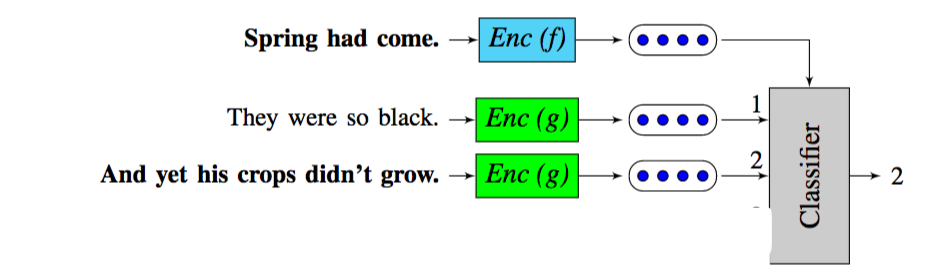
\includegraphics[width=0.9\textwidth]{fig1_architecture}
\subcaption{Figure taken from \cite{eff_framework}}

\end{subfigure}
\begin{subfigure}[c]{0.4\textwidth}

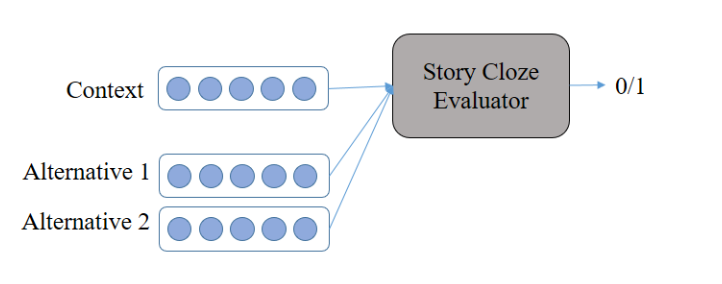
\includegraphics[width=0.9\textwidth]{fig2_architecture}
\subcaption{Figure taken from \cite{mostafazadeh-EtAl:2016:RepEval}}

\end{subfigure}
\caption{{\bf Frage: }Welche Art von Grafik ist für den Report geeigneter (links: m\"usste ich noch anpassen auf unsere Methode -NEIN, nicht anpassen, siehe oben; die Grafik rechts k\"onnte man so \"ubernehmen - diese Grafik sagt nichts relevantes ueber unseren Ansatz aus.}
\end{figure}



\section{Training}
For trainable word embeddings, we based on with GloVe pre-trained word embeddings in 300 dimensions \cite{pennington2014glove}. 
As training data, we exclusively used the given corpus of $88161$ five sentence stories. In these stories, there were no alternative (wrong) ending sentences. 
A context scope of +/- 1  was used, where the previous and the next sentences are predicted given an input sentence.
After measuring accuracy on the validation set, we chose hyperparameters to be a minibatch size of 100 sentences (i.e. 20 cloze stories with 5 sentences each) with a dropout rate of 0.25. We trained over 5 epochs to minimize cross-entropy with Adam Optimizer at a learning rate of 1e-3.
Due to the efficient nature of this approach, total training time on a single GTX 1080 Ti GPU was well under an hour.


\section{Experiments}
On the given validation set, we achieve an accuracy of $0.612$ using the parameters mentioned above. This result is comparable with respect to what has been published earlier \cite{}.

\section{Conclusion}
Due to the limited scope and time of this project, we felt we couldn't fully exploit the benefits of our chosen approach. For further investigation, the use of more sophisticated embeddings (case senstive; Skip-thoughts) as well as using more sophisticated RNN encoding functions look promising.

%\bibliographystyle{plain}
\bibliography{bibliography} 
\end{document}
